\documentclass{beamer}
\usepackage{graphicx}
\newcommand{\quotes}[1]{``#1''}
\graphicspath{ {./images/} }
\mode<presentation>
\title{Properties contaminated with oil - investment scenarios}
\author{Dinkar Ganti}
\begin{document}
\begin{frame}
  \titlepage
\end{frame}
\begin{frame}
\frametitle{Tasks}
\section{Tasks}
  The number of tasks to cleanup a property can spread out over weeks or months and therefore it is important to list them and manage them. Here we list a subset of tasks that need to be caputured in the current real world.
  \begin{itemize}
    \item Baseline analysis or site characterization --- estimated between 5000 - 20000 USD.
    \item Case manager's assessment of the property to provide cleanup guidance.
    \item Environment consultant's cleanup plan.
    \item Environment consultant's rate list as per DEP's desirable rate list per task. 
    \item Installation of cleanup and monitoring equipment.
    \item Maintainence of currency of insurance documents.
    \item Workers liability
    \item Attorneys signoff for task if needed.
    \item Escrow accounts : in real life such account are needed. (note: in a trustless environment these accounts are simpler to setup).
  \end{itemize}
\end{frame}
\begin{frame}
\frametitle {Glossary}
\section{Glossary}
As in any field the field of contamination remediation is full of jargon that can be mind-numbing at times. Here we try to cover some of the terms to help bridge the gap.
\begin{itemize}
  \item DEP --- The department of environment protection is a state agency in the United States that has complete jurisdiction on the cleanup plan process and approval of an tasks that need to be completed as part of the cleanup. 
  \item NFA --- Short for No Further Action. This document usually ties to any lien the DEP may have on the property. An NFA implies that the property is free from contamination and the relevant case is closed. For the investor it means that the property can be resold at prices comparable to similar properties in the neighborhood.
  \item USEPA --- United States Environment Protection Agency. An agency with a global directive on environment law covering soil, water and air within the 48 states, Alaska and Hawaii. Despite such a title, the USEPA's involvement in properties is limited for most properties partly due to states rights (need to confirm this) and when they do get involved the sites are usually declared as brownfields and have a different source of funding as well as jurisdiction, which we will cover in a later section \ref{brownfields} on Brownfields.
\end{itemize}
\end{frame}

\begin{frame}
\frametitle{Where is the opportunity}
\section {Opportunity}
Usually these properties are written-off by the property owners as the costs of cleanup for even a relatively minor spill can go upwards of USD 40000 (empirical evidence). The purpose of realitz is to bring together innovative solution providers with investors to realize the potential increase in the value of a property contaminated with oil after an effective cleanup. Formula for evaluating the potential increase of the value of a property needs to account for a few principles, namely the value of the property after cleanup is capped by the comparables in the market and the risk of cleanup needs to be assumed to be infinite, analogous to the risk of an option writer in the regulated options exchange. In other words, the users of this application will be a community of solution providers with sufficient experience and a trackrecord as well as investors and other parties involved. It is likely that investors will lose their investment (full disclosure). The purpose of this application is not to discuss the merits of an investment or a solution. The purpose of this application is to present with an immutable ledger of events and a place to contractually manage tasks involving their properties.

The keyword here is innovative and usually investors see RED for every innovative solution to save them some money. This fear and mistrust can be addressed by having a trustless system to effectively cleanup a property.
\end{frame}
\begin{frame}
\frametitle{Brownfields}
\section{Brownfields} \label{brownfields}
  TBD.
\end{frame}

\begin{frame}
\frametitle{TLDR}
\section{TLDR}
  When a release is reported for a property that triggers a set of actions by parties involved due to the liabilities that are ensuant to the release. For example, if the spill is greater than 50 gallons in the state of Virginia, the release is treated as an emergency with a DEP case number assigned. For example,the image shown above describes the closure of a dep case file and the reasons for the closure. More details are outlined in the actual report though, for the purposes of this discussion we the limit our attention to the phrase \quotes{according to state law}, as this encompasses the level of scrutiny each property receives from the relevant DEP (Department of Environment Protection, usually a state regulatory body). The current process is quite labor-intensive and requires a level of effort from many parties including and not limited to the case managers attention to the project plan, the validity of the licenses of the environment contractors, the property owner, the property owner's insurance company and is quite detailed. Each party needs to manage its own part of the project to ensure a timely closure. As we can clearly see that this process needs to be supplemented with a trustless process so that no party has an opportunity to change their mind or data as well as be availble for easy access after a particular task and its associated data have been uploaded on the blockchain.
  
\end{frame}

\begin{frame}
\frametitle{TLDR2}
\section {TLDR2}
  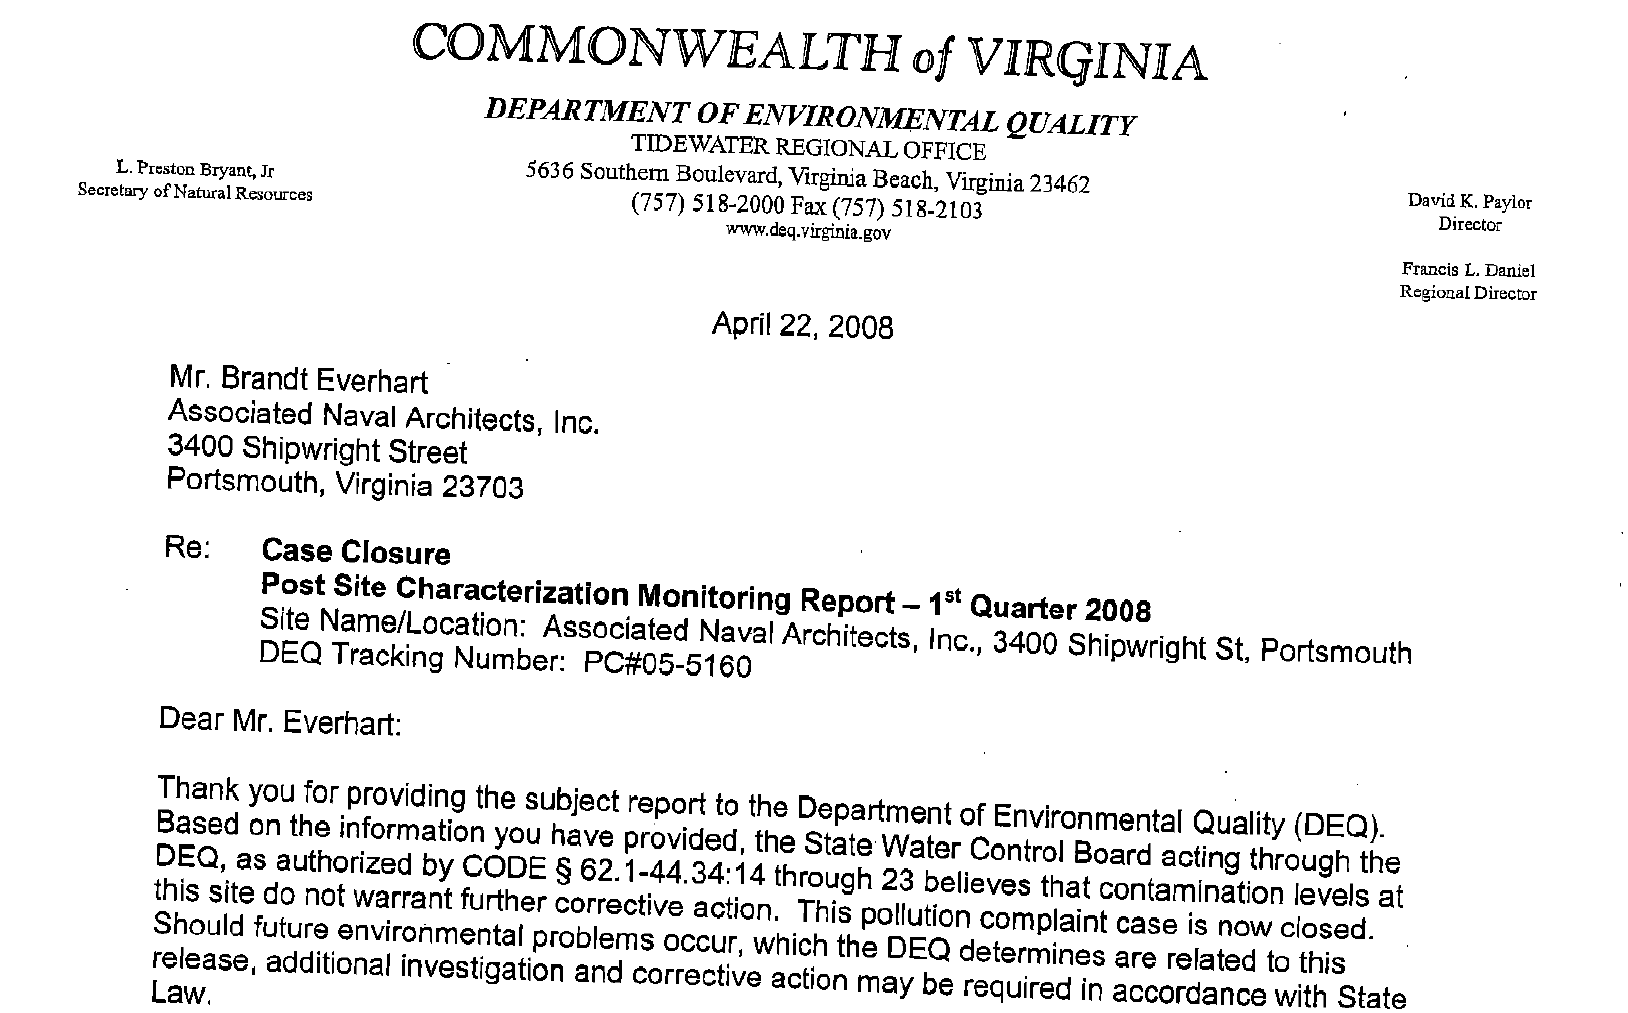
\includegraphics[width = 4in, height = 4in]{vadeqnfa}
\end{frame}
\end{document}